%%%%%%%%%%%%%%%%%%%%%%%%%%%%%%%%%%%%%%%%%%%%%%%%%%%%%%%%%%%%%%%%%
% Dissertacao de Mestrado / Dept Fisica, CFM, UFSC              %
% Andre@UFSC - 2011                                             %
%%%%%%%%%%%%%%%%%%%%%%%%%%%%%%%%%%%%%%%%%%%%%%%%%%%%%%%%%%%%%%%%%


%:::::::::::::::::::::::::::::::::::::::::::::::::::::::::::::::%
%                                                               %
%                          Capítulo 4                           %
%                                                               %
%:::::::::::::::::::::::::::::::::::::::::::::::::::::::::::::::%

%***************************************************************%
%                                                               %
%                       Análise da Amostra                      %
%                                                               %
%***************************************************************%

\chapter{Análise da amostra \STARLIGHTUV}
\label{sec:Analise}


%***************************************************************%
%                                                               %
%                  Análise - Diagrama cor -- cor                %
%                                                               %
%***************************************************************%

\section{Diagrama cor--cor}

De posse de uma amostra de galáxias com uma informação adicional (as magnitudes
em ultravioleta), é natural tentar ver como estas novas medidas se relacionam às
medidas conhecidas. \citet{Chilingarian2011} mostram que, num gráfico
tridimensional das cores $\mathrm{NUV}-r$ e $g-r$ contra a magnitude $z$, a
distribuição de galáxias pode ser aproximada por uma superfície polinomial de
baixa ordem. Os autores mostram que há uma forte correlação entre a cor
$\mathrm{NUV}-r$ e a morfologia da galáxia. Eles também estudam o histórico de
formação estelar (SFH) no diagrama $\mathrm{NUV}-r$ contra $g-r$, mas a
exploração é um tanto superficial.

\begin{figure}
	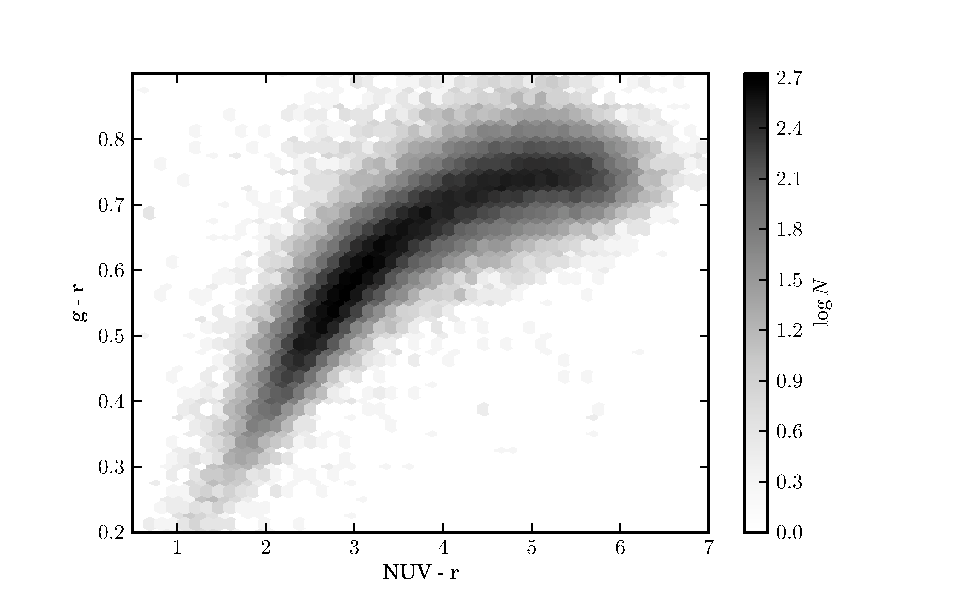
\includegraphics{figuras/uvcolor-color-density.eps}
	\caption[Densidade de galáxias no diagrama cor--cor UV.]
	{Densidade de galáxias em função de cor UV ($\mathrm{NUV}-r$) e cor óptica
	($g-r$). A intensidade dos bins hexagonais é o logaritmo do número de pontos
	dentro do bin, para melhorar a visualização. Esta figura é similar à figura 4
	de \citet{Chilingarian2011}. Foram selecionados objetos da amostra do
	\starlight com magnitude na banda $z$ entre $-23$ e $-21,5$ e {\em redshift}
	entre $0,04$ e $0,17$. As magnitudes $g$, $r$ e $z$ são do \SDSS.}
	\label{fig:DensityColor}
\end{figure}

A figura \ref{fig:ColorStarlightParam} mostra as propriedades físicas das
galáxias obtidos através do \starlight no diagrama cor--cor. Os eixos são os
mesmo da figura \ref{fig:DensityColor}, com a cor dos pontos indicando o valor
de cada parâmetro. \citeauthor{Chilingarian2011} chegam numa relação semelhante
à do painel (a) para a idade das SSP, porém através de outros meios. Estas
propriedades físicas são vistas com mais detalhes na seção
\ref{sec:Analise:PropFisicas}.

\begin{figure}
	\includegraphics{figuras/uvcolor-color.eps}
	\caption[Diagrama cor--cor UV para os diversos parâmetros \starlight.]
	{Propriedades físicas das galáxias em função de cor UV e cor óptica. O contorno
	das figuras representam os níveis referentes à figura \ref{fig:DensityColor},
	e os eixos horizontal e vertical são os mesmos. As cores dos pontos nos painéis
	correspondem a: \textbf{(a)} Logaritmo da idade média das SSP componentes da
	galáxia, ponderada pelo fluxo. \textbf{(b)} O mesmo que a anterior, mas
	ponderada pela massa. \textbf{(c)} Metalicidade média das SSP componentes da
	galáxia, ponderada pelo fluxo. \textbf{(d)} O mesmo que a anterior, ponderada
	pela massa. \textbf{(e)} Logaritmo da massa estelar da galáxia, em massas
	solares. \textbf{(f)} Extinção por poeira na galáxia, na banda $V$.}
	\label{fig:ColorStarlightParam}
\end{figure}


%***************************************************************%
%                                                               %
%                     Análise - Classificação                   %
%                                                               %
%***************************************************************%

\section{Classificação das galáxias}

Nesta seção são discutidas formas de classificação de galáxias, e a forma como a
cor UV das galáxias está relacionada às classes. São utilizadas as linhas de
emissão \Halpha, \Hbeta, \NII e \OIII (daqui em diante chamados apenas de \nII e
\oIII).

A classificação feita a seguir divide as galáxias em dois grupos principais: as
galáxias com linha de emissão (ELG) e as galáxias passivas (PG). As ELG ainda
podem ser divididas dependendo do processo físico pro trás das linhas de
emissão. Essencialmente, os agentes ionizantes responsáveis pelas linhas
observadas em galáxias são estrelas jovens, núcleos ativos e objetos do tipo
HOLMES ({\em Hot Low-Mass Evolved Stars}). \citet{CidFernandes2011} elabora um
procedimento simples para separar as galáxias em classes, de acordo com o agente
ionizante que domina a emissão de linhas na galáxia. A distinção é feita de
acordo com a largura equivalente da linha \Halpha ($\WHa$) e a razão entre o
fluxo de linhas $\nII/\Halpha$, num diagrama conhecido como WHAN. Este diagrama
relaciona duas quantidades físicas diferentes: $\WHa$ mede a quantidade de
fótons ionizantes absorvida pelo gás em relação à massa estelar, e
$\nII/\Halpha$ mede a abundância de nitrogênio, o estado de ionização e a
temperatura do gás. Assim, as galáxias são separadas em classes neste diagrama
conforme os seguintes critérios:

\begin{list}{}{\setlength\itemsep{0pt}}
\item \textbf{(a)} Galáxias com formação estelar (SFG): $\log(\nII/\Halpha) <
-0,4$ e $\WHa > 3\text{\AA}$,
\item \textbf{(b)} Galáxias com núcleo ativo forte (sAGN): $\log(\nII/\Halpha) >
-0,4$ e $\WHa > 6\text{\AA}$,
\item \textbf{(c)} Galáxias com núcleo ativo fraco (wAGN): $\log(\nII/\Halpha) >
-0,4$ e $3\text{\AA} > \WHa > 6\text{\AA}$,
\item \textbf{(d)} Galáxias ``aposentadas'' (RG): $\WHa < 3\text{\AA}$,
\item \textbf{(e)} Galáxias passivas (PG): $\WHa < 0,5\text{\AA}$ e $\WnII <
0,5\text{\AA}$.
\end{list}

O diagrama WHAN para a amostra \starlightUV pode ser visto na figura
\ref{fig:Whan}. A cor dos pontos para cada classe é o mesmo utilizado por
\citet{CidFernandes2011}. São $45\,086$ galáxias com formação estelar, $32\,491$
galáxias com núcleo ativo forte, $12\,003$ galáxias com núcleo ativo fraco,
$24\,439$ galáxias aposentadas e $13\,483$ galáxias passivas. O mesmo diagrama,
porém com a cor dos pontos representando a cor $\mathrm{NUV}-r$ das galáxias
(figura \ref{fig:WhanUV}), mostra que a cor UV das galáxias está relacionada à
sua classe.

\begin{figure}
	\includegraphics{figuras/whan.eps}
	\caption[Diagrama de diagnóstico WHAN.]
	{Diagrama de diagnóstico WHAN. As linhas tracejadas separam as galáxias
	em classes. \textbf{Azul}: galáxias com formação estelar (SFG). \textbf{Verde
	claro}: galáxias com núcleo ativo forte (sAGN). \textbf{Verde forte}:
	galáxias com núcleo ativo fraco (wAGN). \textbf{Preto}: galáxias aposentadas
	(RG). \textbf{Vermelho}: galáxias passivas (PG). \textbf{Magenta}: Galáxias
	que não se encaixam em nenhuma destas classes.}
	\label{fig:Whan}
\end{figure}

\begin{figure}
	\includegraphics{figuras/whan-uv.eps}
	\caption[Cores UV no diagrama WHAN.]
	{Diagrama WHAN semelhante ao da figura \ref{fig:Whan}. A cor dos pontos
	representa $\mathrm{NUV}-r$. Pode-se notar que a cor UV das galáxias é
	diferente para cada classe.}
	\label{fig:WhanUV}
\end{figure}

Outra forma de classificar as galáxias é através das razões entre linhas de
emissão $\nII/\Halpha$ e $\oIII/\Hbeta$. Este diagrama, conhecido como BPT
\citep{Baldwin1981} é bastante utilizado na astronomia extragalática. Em
\citet{CidFernandes2010} discute-se os detalhes da classificação das galáxias
classificação utilizando o diagrama BPT. As linhas tracejadas separam as
galáxias nas classes {\em Seyfert} (que corresponde à classe sAGN na
classificação pelo WHAN), {\em LINER} (correspondente às wAGN e aposentadas) e
galáxias de formação estelar (SFG). A cor UV das galáxias da amostra no diagrama
BPT (figura \ref{fig:BPTUV}) é consistente com as cores para o diagrama WHAN.

\begin{figure}
	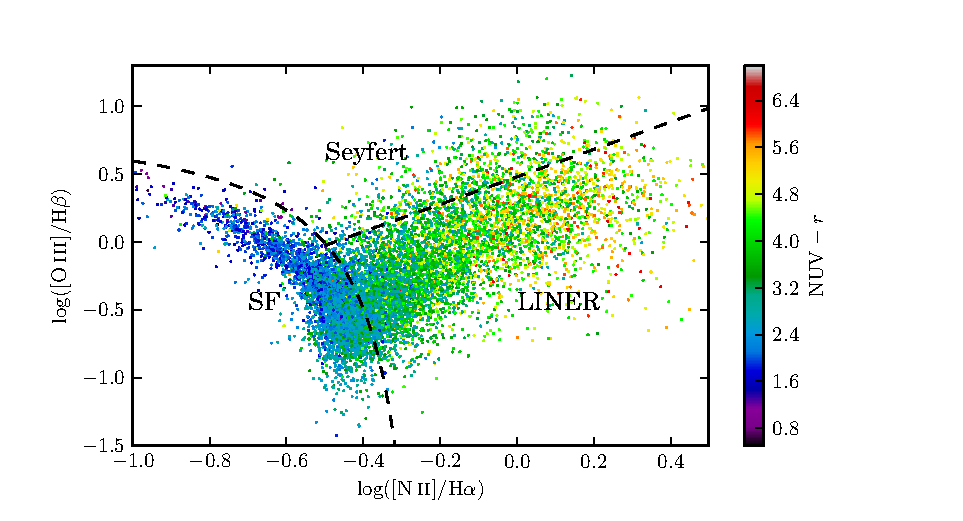
\includegraphics{figuras/bpt-uv.eps}
	\caption[Cores UV no diagrama BPT.]
	{Diagrama BPT, também usado para classificar galáxias. A cor dos
	pontos representa $\mathrm{NUV}-r$. As linhas tracejadas separam das galáxias nas
	classes {\em Seyfert}, {\em LINER} e formação estelar, conforme
	\citet[linhas S06 e K06 da tabela 1]{CidFernandes2010}. A cor UV das galáxias
	em cada classe é consistente com a classificação usando WHAN.}
	\label{fig:BPTUV}
\end{figure}

As classes de galáxias ocupam regiões distintas do diagrama cor--cor. Na figura
\ref{fig:ColorClass} a cor dos pontos representa a classe das galáxias da mesma
forma que na figura \ref{fig:Whan}. Embora não esteja muito claro para as RG e
PG, as classes formam uma sequência neste diagrama. Isto pode ser visto mais
facilmente na figura \ref{fig:HistogramaCorClasse}. Esta figura é de certo modo
uma versão resumida da figura \ref{fig:ColorClass}. Mesmo havendo uma
sobreposição considerável ente as classes, a sequência está bem definida.

% FIXME: Explicar por que chamar RG de azul em UV.
É interessante notar que a separação entre as classes é mais pronunciada em UV.
As classes RG e PG mal se distinguem no óptico, enquanto que em UV as RG se
mostram consistentemente mais azuis\footnote{Azul em ultravioleta?\fixme}.
Através de uma inspeção visual pode-se inferir, ainda que qualitativamente, que
as distribuições em UV são significativamente assimétricas em comparação com as
distribuições no óptico. Isto pode se um indício de uma contaminação entre as
classes, evidenciada agora pelos novos dados em UV. No entanto é necessário
fazer um estudo com base estatística.

\begin{figure}
	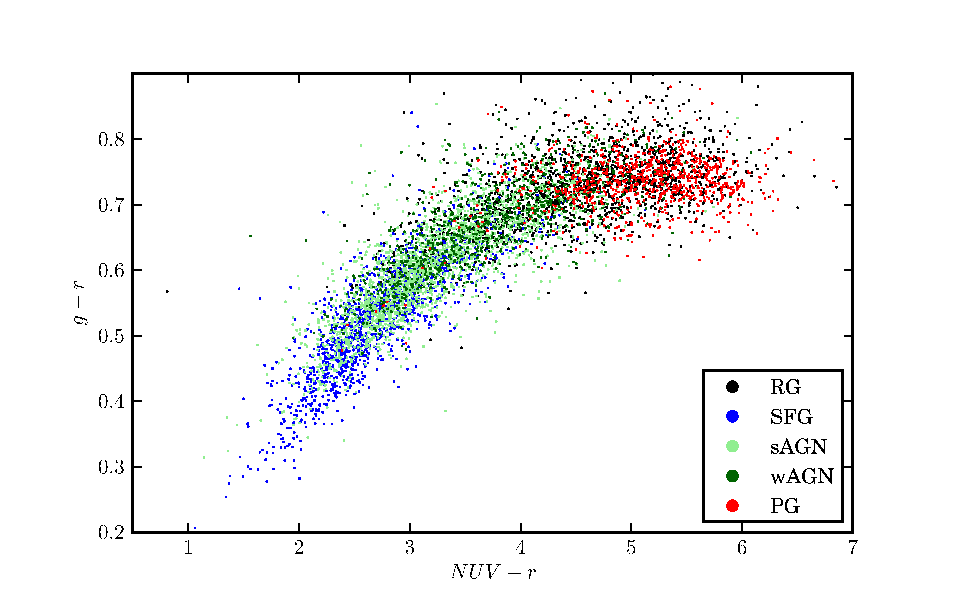
\includegraphics{figuras/uvcolor-color-class.eps}
	\caption[Diagrama cor--cor UV de acordo com o tipo de galáxia.]
	{Classes de galáxias no diagrama cor--cor UV. As cores referentes às classes de
	galáxia são as mesmas do diagrama WHAN (figura \ref{fig:Whan}). É possível
	notar uma separação entre as classes, embora não tão clara quanto no diagrama
	WHAN.}
	\label{fig:ColorClass}
\end{figure}

\begin{figure}
	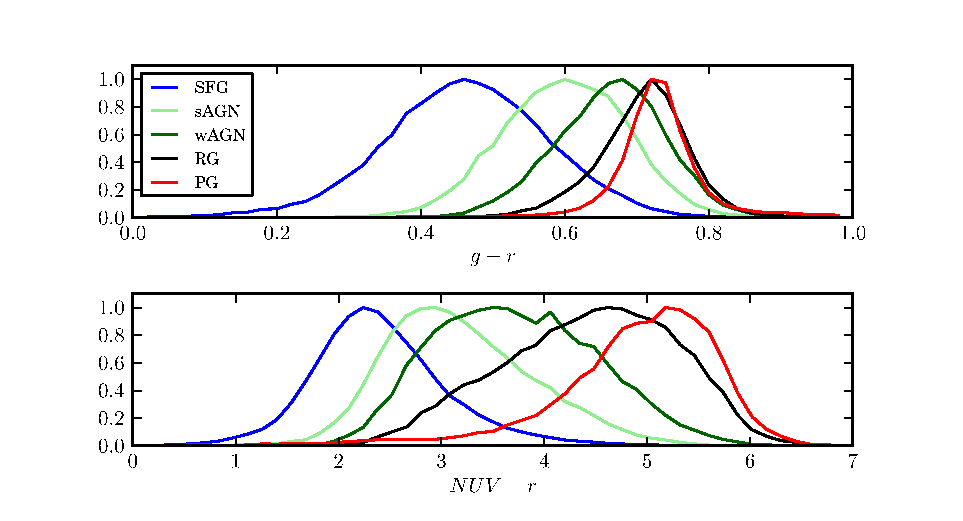
\includegraphics{figuras/histo_galtype_color.eps}
	\caption[Histogramas de cores para as classes de galáxias.]
	{Histogramas normalizado das cores óptica ($g-r$) e ultravioleta
	($\mathrm{NUV}-r$) para as classes de galáxias. A cor das linhas representa a
	classe conforme a figura \ref{fig:Whan}. Em ultravioleta a separação entre as
	classes de galáxias aposentadas (RG) e passivas (PG) torna-se mais clara. Note
	que os histogramas seguem o agrupamento das classes na figura
	\ref{fig:ColorClass}.}
	\label{fig:HistogramaCorClasse}
\end{figure}


%***************************************************************%
%                                                               %
%          Análise - Pro. Físicas no diagrama cor -- cor        %
%                                                               %
%***************************************************************%

\section{Propriedades físicas no diagrama cor--cor}
\label{sec:Analise:PropFisicas}

% TODO: Parâmetros físicos das galáxias no diagrama de cores.
TODO: Parâmetros físicos das galáxias no diagrama de cores. A sequência de
classes no diagrama cor--cor. Figura \ref{fig:ATFluxColor}.

Visto que os agentes por trás das linhas de emissão das galáxias são
fundamentalmente diferentes (estrelas jovens, núcleos ativos e HOLMES) para
cada classe, é de se esperar que as propriedades físicas das galáxias sejam
diferentes para ca


A classificaão das galáxias na seção anterior\ldots As propriedades físicas das
galáxias estão relacionadas à sua classe\ldots

AV pode ser negativo?

\begin{figure}
	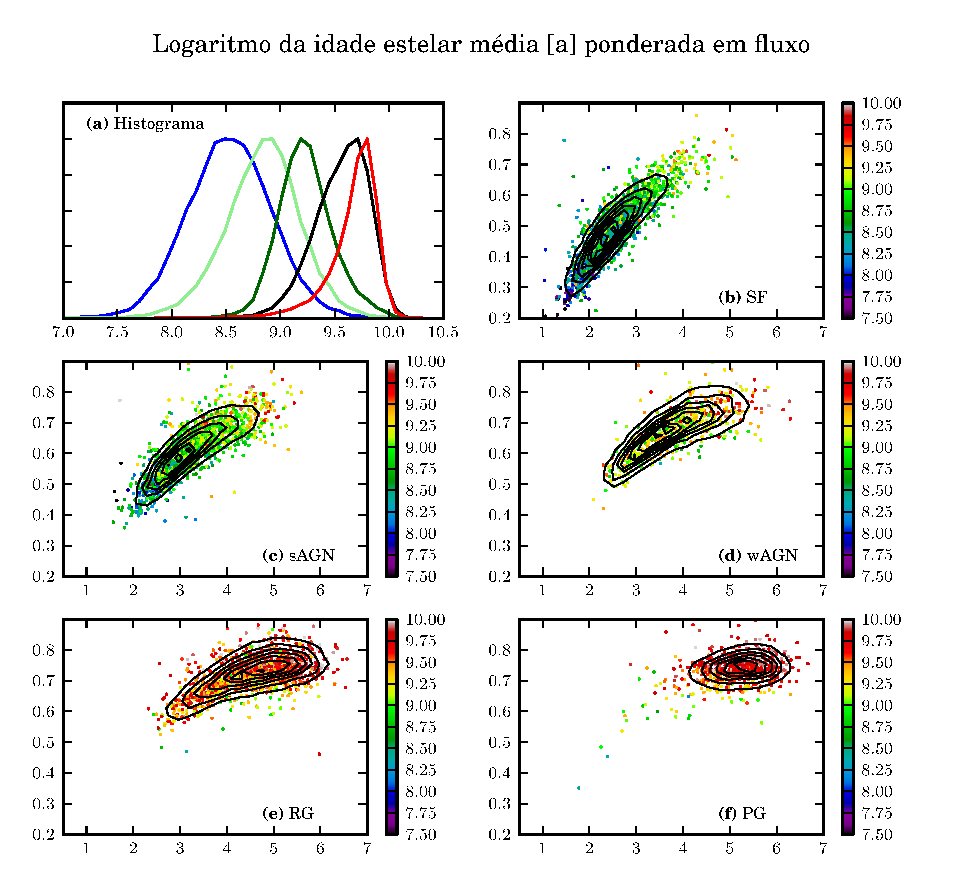
\includegraphics{figuras/uvcolor-color-at_flux-byclass.eps}
	\caption[Idade média das SSP ponderada em fluxo no diagrama cor--cor UV.]
	{Idade média das SSP componentes das galáxias ponderada pelo fluxo, em função
	de $\mathrm{NUV}-r$ e $g-r$. O painel \textbf{(a)} contém todas as galáxias da
	amostra. Os painéis de \textbf{(b)} a \textbf{(f)} contém somente as galáxias
	com formação estelar (SFG), AGN fortes (sAGN), AGN fracas (wAGN), galáxias
	aposentadas (RG) e galáxias passivas (PG), respectivamente. Os contornos
	indicam a densidade de galáxias. A idade média da distribuição vai aumentando
	conforme a classe, na sequência apresentada.}
	\label{fig:ATFluxColor}
\end{figure}

\begin{figure}
	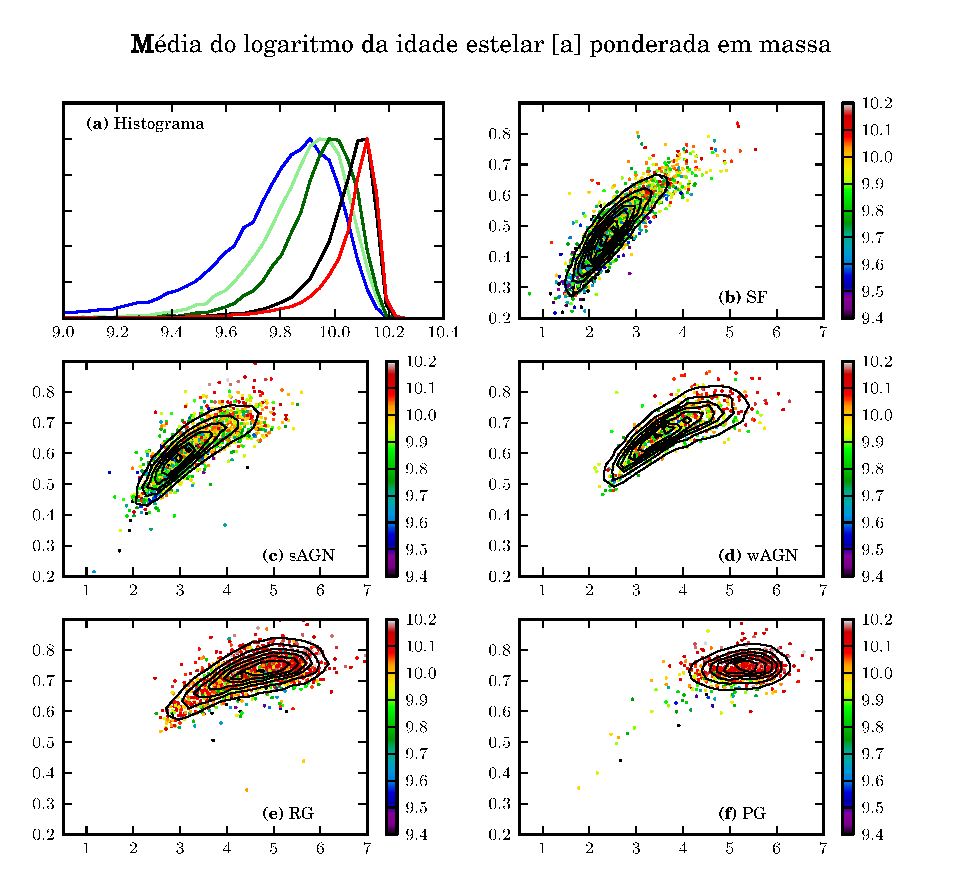
\includegraphics{figuras/uvcolor-color-at_mass-byclass.eps}
	\caption[Idade média das SSP ponderada em massa no diagrama cor--cor UV.]
	{O mesmo que a figura \ref{fig:ATFluxColor}, para a idade média das SSP
	componentes das galáxias, ponderada pela massa. Note que a escala de idades não
	é a mesma.}
	\label{fig:ATMassColor}
\end{figure}

\begin{figure}
	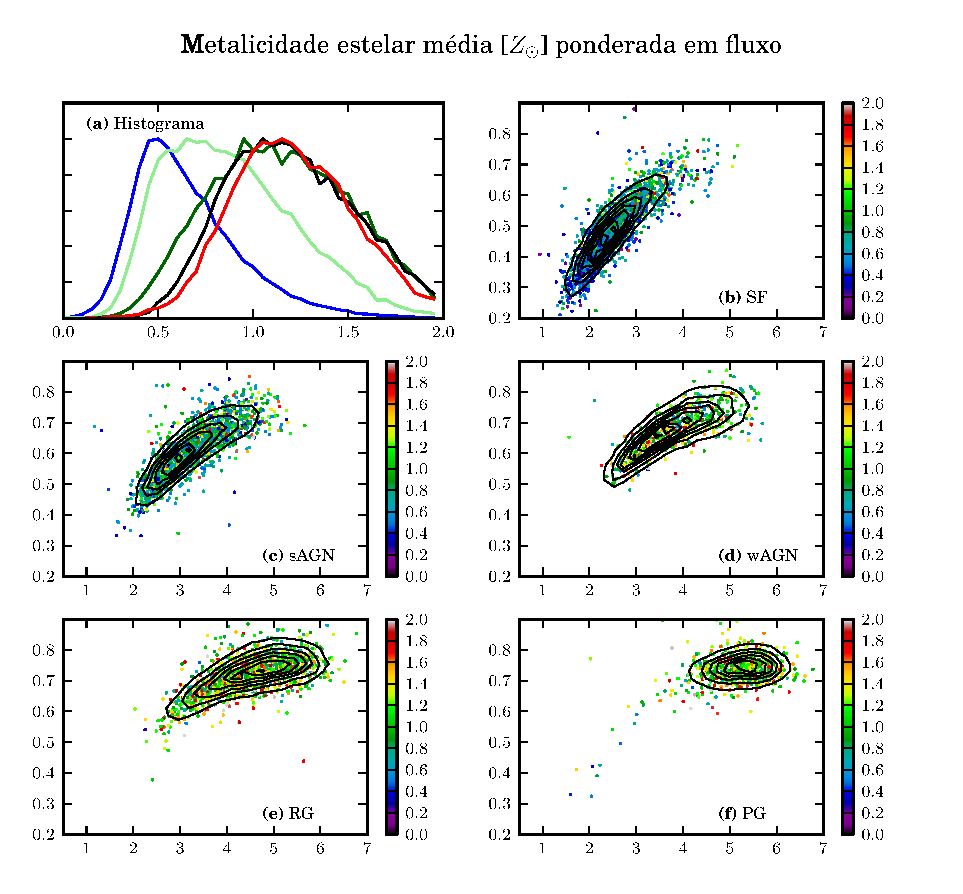
\includegraphics{figuras/uvcolor-color-am_flux-byclass.eps}
	\caption[Metalicidade média das SSP ponderada em fluxo no diagrama cor--cor
	UV.]
	{O mesmo que a figura \ref{fig:ATFluxColor}, para a metalicidade média das
	SSP componentes das galáxias, ponderada pelo fluxo.}
	\label{fig:AMFluxColor}
\end{figure}

\begin{figure}
	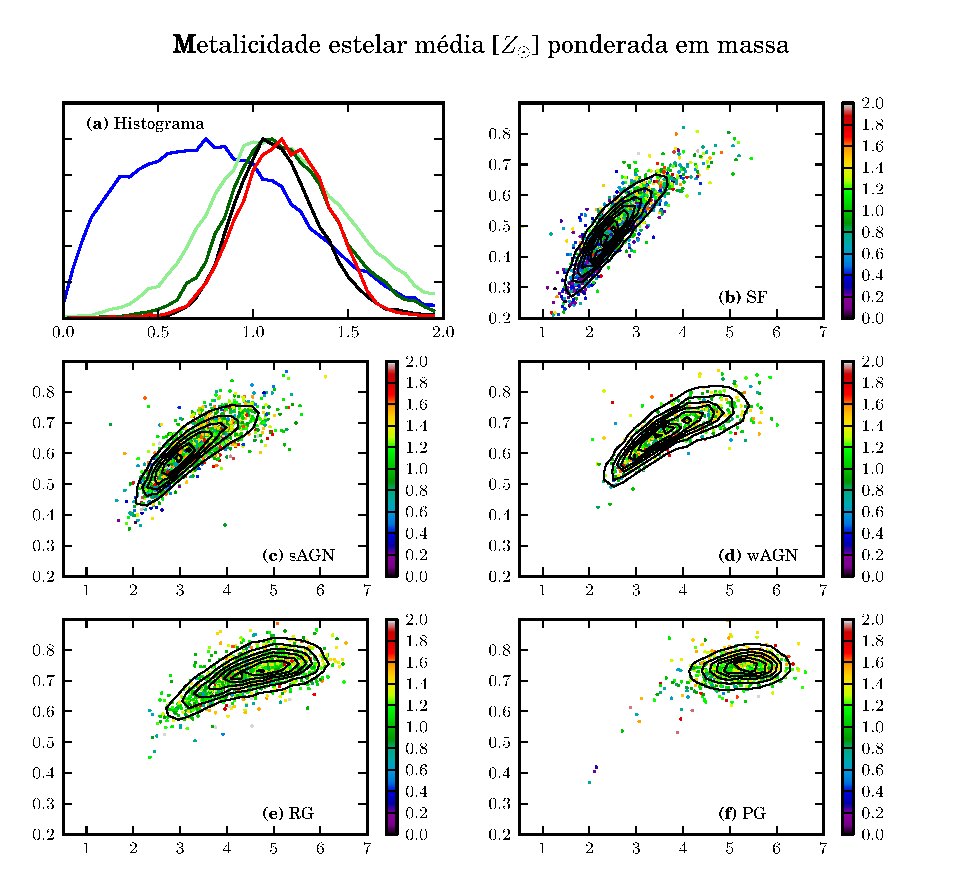
\includegraphics{figuras/uvcolor-color-am_mass-byclass.eps}
	\caption[Metalicidade média das SSP ponderada em massa no diagrama cor--cor
	UV.]
	{O mesmo que a figura \ref{fig:ATFluxColor}, para a metalicidade média das
	SSP componentes das galáxias, ponderada pelo massa.}
	\label{fig:AMMassColor}
\end{figure}

\begin{figure}
	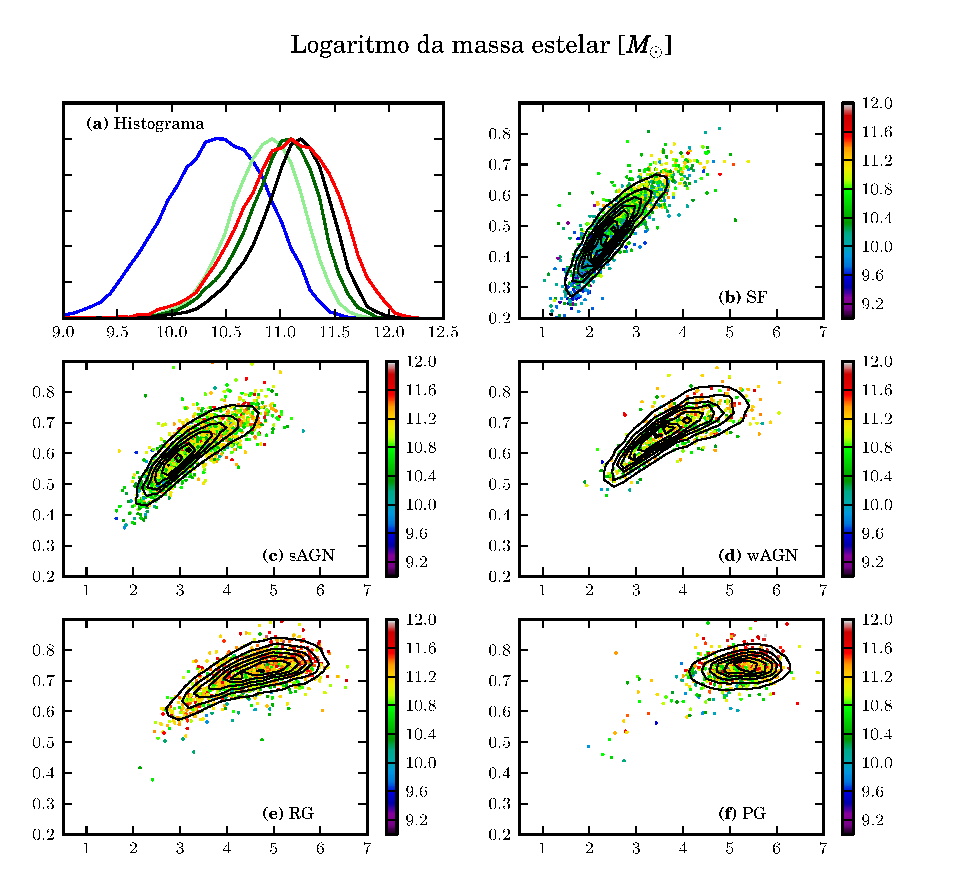
\includegraphics{figuras/uvcolor-color-mcor_gal-byclass.eps}
	\caption[Massa estelar das galáxias no diagrama cor--cor UV.]
	{O mesmo que a figura \ref{fig:ATFluxColor}, para o logaritmo da massa estelar
	das galáxias em massas solares.}
	\label{fig:MCorGalColor}
\end{figure}

\begin{figure}
	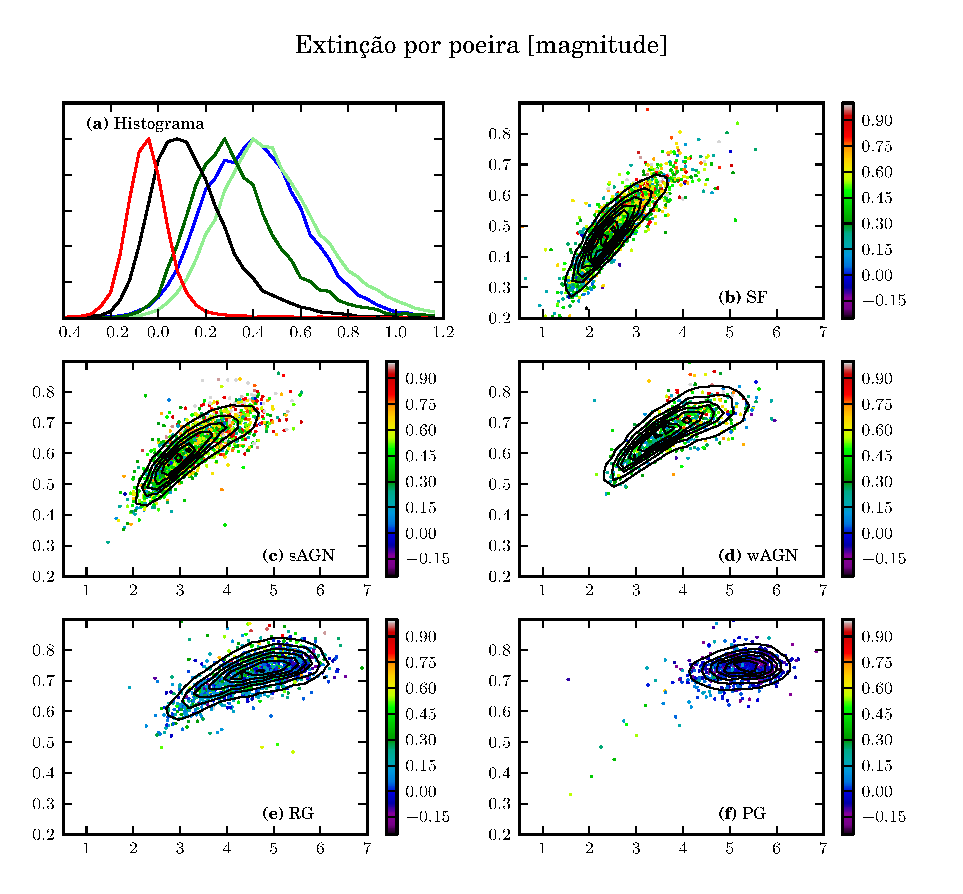
\includegraphics{figuras/uvcolor-color-AV-byclass.eps}
	\caption[Extinção por poeira no diagrama cor--cor UV.]
	{O mesmo que a figura \ref{fig:ATFluxColor}, para a extinção por
	poeira na banda $V$ das galáxias.}
	\label{fig:AVColor}
\end{figure}

\begin{figure}
	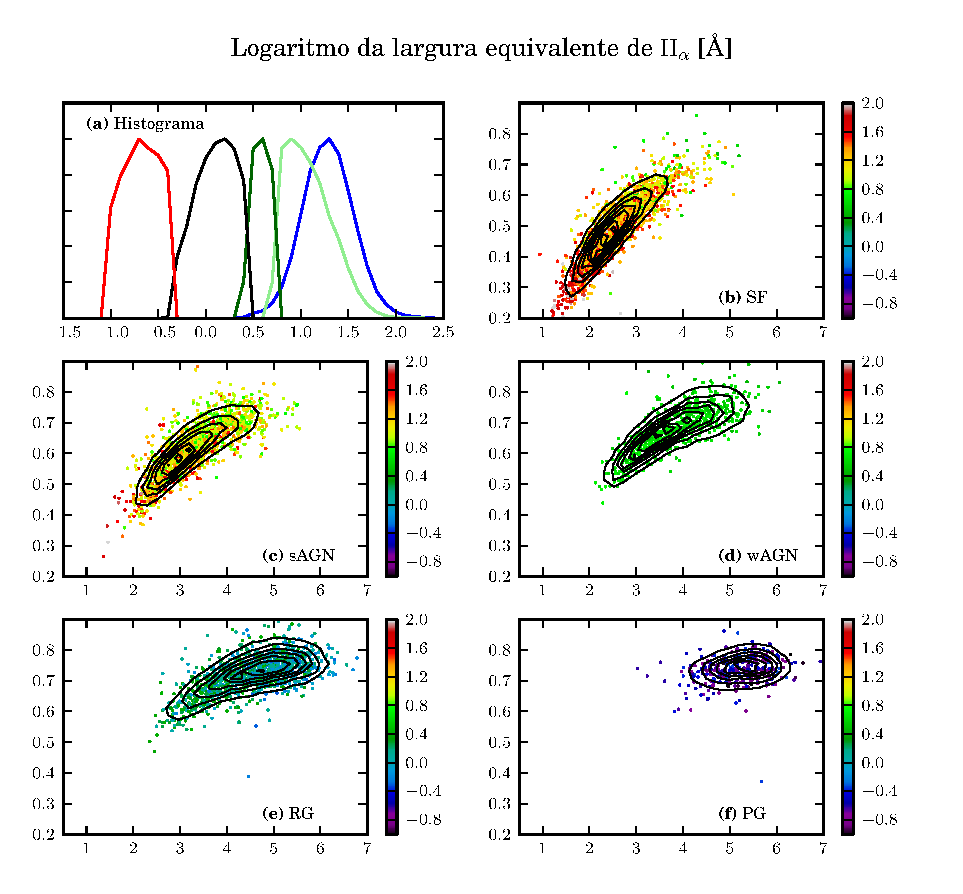
\includegraphics{figuras/uvcolor-color-halpha_ew-byclass.eps}
	\caption[Largura equivalente de \Halpha no diagrama cor--cor UV.]
	{O mesmo que a figura \ref{fig:ATFluxColor}, para o logaritmo da largura
	equivalente de \Halpha das galáxias.}
	\label{fig:EWHaColor}
\end{figure}

\section{Discussão}

\subsection{A separação entre galáxias aposentadas e passivas}

%TODO: Comparar galáxias aposentadas com passivas
TODO: Comparar galáxias aposentadas com passivas.

%\backslash citep[In prep. perpetuum]${$Mateus2013$}$.
\textbackslash{}citep{[In prep. perpetuum]}\{Mateus2013\}

%citep[In prep. perpetuum]${$Mateus2013$}$.


% End of this chapter
